\let\negmedspace\undefined
\let\negthickspace\undefined
\documentclass[journal,12pt,onecolumn]{IEEEtran}
\usepackage{pgfplots}
\pgfplotsset{compat=1.17}
\usepackage{cite}
\usepackage{amsmath,amssymb,amsfonts,amsthm}
\usepackage{algorithmic}
\usepackage{graphicx}
\usepackage{textcomp}
\usepackage{xcolor}
\usepackage{txfonts}
\usepackage{listings}
\usepackage{enumitem}
\usepackage{mathtools}
\usepackage{gensymb}
\usepackage{comment}
\usepackage[breaklinks=true]{hyperref}
\usepackage{tkz-euclide} 
\usepackage{listings}
\usepackage{gvv}                                        
\def\inputGnumericTable{}                                 
\usepackage[latin1]{inputenc}                                
\usepackage{color}                                            
\usepackage{array}                                            
\usepackage{longtable}                                       
\usepackage{calc}                                             
\usepackage{multirow}                                         
\usepackage{hhline}                                           
\usepackage{ifthen}                                           
\usepackage{lscape}
\newtheorem{theorem}{Theorem}[section]
\newtheorem{problem}{Problem}
\newtheorem{proposition}{Proposition}[section]
\newtheorem{lemma}{Lemma}[section]
\newtheorem{corollary}[theorem]{Corollary}
\newtheorem{example}{Example}[section]
\newtheorem{definition}[problem]{Definition}
\newcommand{\BEQA}{\begin{eqnarray}}
\newcommand{\EEQA}{\end{eqnarray}}
\newcommand{\define}{\stackrel{\triangle}{=}}
\theoremstyle{remark}
\newtheorem{rem}{Remark}
\begin{document}
\bibliographystyle{IEEEtran}
\vspace{3cm}
\title{GATE GE 81Q}
\author{EE23BTECH11021 - GANNE GOPI CHANDU$^{*}$% <-this % stops a space
}
\maketitle
\bigskip
\renewcommand{\thefigure}{\theenumi}
\renewcommand{\thetable}{\theenumi}
\bibliographystyle{IEEEtran}
\textbf{Question}\\
The value of the convolution of $f(x) = 3\cos(2x)$ and $g(x) = \frac{1}{3}\sin(2x)$ where $x \in [0, 2\pi)$, at $x = \frac{\pi}{3}$, is (Rounded off to 2 decimal places)\\
\textbf{Solution}\\
The Fourier transform of given functions is
 \begin{align}
        F(\omega) &= \mathcal{F}[f(x)] = 3{\pi}[\delta(\omega - 2\pi) + \delta(\omega + 2\pi)] \\
        G(\omega) &= \mathcal{F}[g(x)] = \frac{\pi}{3}[\delta(\omega - 2\pi) - \delta(\omega + 2\pi)]
 \end{align}
Multiply the $F(\omega)$ and $G(\omega)$
\begin{align}
        H(\omega) &= F(\omega) \cdot G(\omega) \\
        &= 3{\pi} \cdot \frac{\pi}{3}[\delta(\omega - 2\pi) + \delta(\omega + 2\pi)] \cdot [\delta(\omega - 2\pi) - \delta(\omega + 2\pi)] \\
        &= {\pi}^2[\delta(\omega - 2\pi) \cdot \delta(\omega - 2\pi) - \delta(\omega - 2\pi) \cdot \delta(\omega + 2\pi) \\
        &\quad + \delta(\omega + 2\pi) \cdot \delta(\omega - 2\pi) - \delta(\omega + 2\pi) \cdot \delta(\omega + 2\pi)] \\
        &= {\pi}^2[\brak{\delta(\omega - 2\pi)}^2 - \brak{\delta(\omega + 2\pi)}^2]\\
        &=0
\end{align}
Take the inverse Fourier Transform
\begin{align}
     h(x) = \mathcal{F}^{-1}[H(\omega)] = 0
\end{align}
So, the convolution of \(f(x)\) and \(g(x)\) at \(x = \frac{\pi}{3}\) is $0$.
\begin{figure}
    \centering
    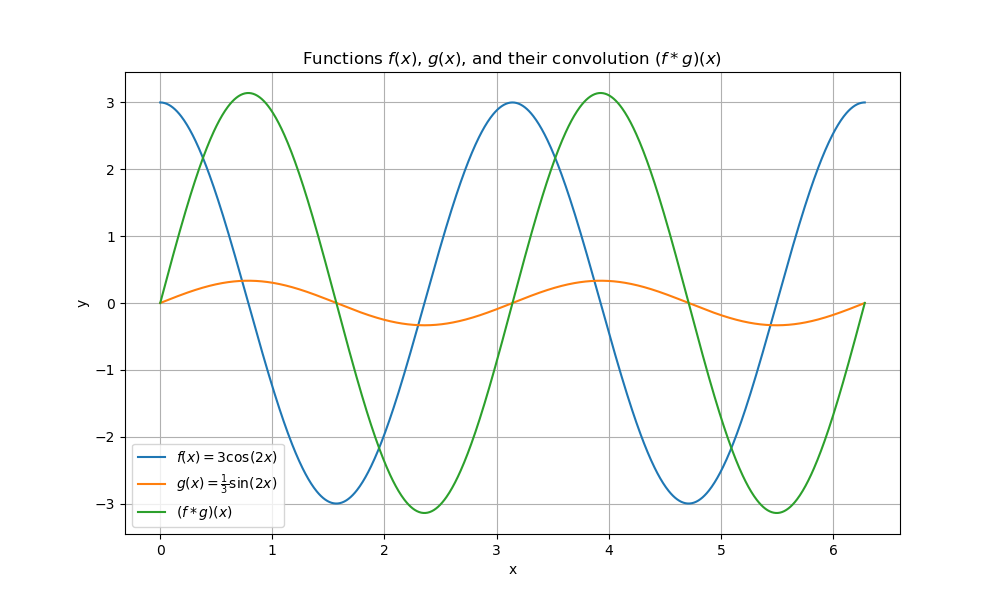
\includegraphics[width=1.0\linewidth]{Figure_3.png}
    \caption{Plot of y vs x}
    \label{fig:2}
\end{figure}\\
\end{document}
